\chapter{Etat de l'art} %20 pages

	% --------------------------------------------------%
	%     												%
	%             Présentation de l'open source			%
	%       										    %
	% --------------------------------------------------%

	\section{Présentation de l'open source} % ready to review

		\subsection{L'open source aujourd'hui}

			\subsubsection{Faire de l'open source c'est ...}

				\paragraph{Un mouvement de pensée\\}

					Le logiciel open source est une affaire de droits. N'importe quel programme devrait être utilisable, modifiable et redistribuable. Les logiciels "propriétaires", portent atteinte à cette philosophie. Le logiciel open source n'est pas une alternative ou bien un autre business model mais une lutte pour cette liberté.

				\paragraph{Un modèle de développement\\}

					L'utilisation d'un modèle de développement open source communautaire est pour Eric \bsc{Raymond} un moyen de démontrer la \textit{supériorité} des logiciels réalisés. Plus que des valeurs éthiques, c'est par la création de ce mouvement avec la fondation de l'\acrshort{osi} qu'Eric \bsc{Raymond} espère imposer l'open source.

				\paragraph{Une dimension humaniste et un patrimoine\\}

					L'open source permet avant tout d'offrir une chance pour les informaticiens futurs de ne pas repartir de zéro, ne pas ré-inventer la roue. Chaque participation de l'Humain apporte sa pierre à l'édifice.
					Selon Smile, la société leader en Europe de l'open source, seulement 10\% d'un code source est issue de notre création pour 90\% de réutilisation de code issus de système d'exploitation, \gls{framework}, et autres composants.

					C'est ici la valeur ajoutée de l'open source. L'informatique progresse essentiellement car le socle de code qui constitue notre patrimoine s'agrandit.

				\paragraph{Respecter des droits\\}

					Les programmes open source ne sont pas des programmes « sans licences » comme on l'entend parfois. C'est au contraire leur licence qui les fait open source. Ils ne sont pas non plus dans le domaine public, c'est à dire n'appartenant à personne en particulier, ou du moins exempts de droits patrimoniaux.\\
					Lorsqu'un développeur écrit un programme, il en détient les droits d'auteur, le « copyright ». Dans certains cas, ce peut être l'entreprise qui l'emploie qui en détient les droits. Et ce copyright peut être vendu, comme bien immatériel, d'une entreprise à une autre.\\

					Le détenteur du copyright est libre de définir l'utilisation qui peut être faite de son programme : 

					\begin{itemize}[label=\textbullet, font=\LARGE \color{burntorange}]
						\item Il peut le garder pour lui, en interdire l'utilisation à qui que ce soit.
						\item Il peut vendre ses droits à un tiers, personne physique ou morale.
						\item Il peut utiliser son droit d'auteur pour préciser les conditions qu'il pose à l'utilisation de son programme. Il écrit ces conditions dans les termes de la licence d'utilisation.
					\end{itemize}
				
					Il est donc important de bien assimiler la logique suivante : à la base de l'open source il y a la licence, et la licence n'existe qu'à partir du droit d'auteur.\\

					Ainsi tous les logiciels open source ont un propriétaire, ils ne sont pas « à personne », ni même « à tout le monde ». Dans certains cas, ce propriétaire peut être une fondation à but non lucratif, ou bien ce peut être une entreprise commerciale ordinaire. Il peut s'agir aussi de plusieurs coauteurs, en particulier à la suite de contributions successives.\\

					Le détenteur des droits est libre de fixer les conditions de licence, il est libre de changer de modèle même (GPL, Affero, AGPL), et il peut y faire des aménagements ou exceptions, ou le diffuser à certains selon une licence, à d'autres selon une autre licence.\\

					Celui qui reçoit le programme, en revanche, n'est pas libre. Il est lié par les termes de la licence. Certes il n'a pas signé de contrat, mais la licence lui a été bien énoncée, et elle stipule qu'il n'a le droit d'utiliser le programme que certaines conditions. S'il refuse ces conditions, il n'a pas le droit d'utiliser le programme. 
					
		\subsection{Les éditeurs open source}

			\subsubsection{Zoom sur l'éditeur}

				L'éditeur, c'est celui qui détient les droits du produit, en assure le développement, la promotion, la diffusion et le support.\\
			
				La seule différence entre l'éditeur propriétaire et l'éditeur open source est que ce dernier publie son produit sous licence open source. Sinon l'investissement dans le développement du produit et son marketing est le même qu'un produit propriétaire.
				Ce modèle a été élu pour permettre de briser les positions acquises d'oligopoles sur le marché du logiciel.
				Il s'agit donc majoritairement de petites entreprises éditrice qui font du support et du développement du produit leur credo.
				Développer un programme open source coûte (un peu) moins cher pour ces entreprises car :

				\begin{enumerate}[font=\color{burntorange}]
		 			\item Elles peuvent s'appuyer sur autant de briques logicielles que la licence leur permet.
		 			\item Elles bénéficient de contributions communautaire.
			 		\item Elles possèdent généralement plus de développeurs passionnés qui participent à son travail.
				\end{enumerate}

				Nous parlerons plus en détail du modèle économique des éditeurs dans la partie sur le marché de l'open source.
				Généralement, l'éditeur fait le choix de partir sur une licence dite GPL car elle présente pour lui deux avantages considérables:

				\begin{enumerate}[font=\color{burntorange}]
		 			\item Du fait de sa popularité, elle est parfaitement lisible et compréhensible ce qui la rend gage de tranparence.
		 			\item Elle empêche les autres de se faire de l'argent sur son dos car elle interdit l'intégration du produit dans un développement propriétaire.
				\end{enumerate}

			\subsubsection{L'aspect communautaire}

				L'éditeur open source a à sa disposition une communauté qui pourra l'aider non seulement dans le support sur les ressources open source qu'il utilise mais également au développement et au support de son oeuvre.

				Au sein de la communauté il est possible de distinguer deux types d'acteurs:

				\begin{description}[font=\color{burntorange}]
					\item[les développeurs indépendants: ] Qu'il s'agisse de gloire, de monté en compétence sur un domaine ou d'altruisme, il existe des développeurs qui soutiennent le développement de produit et participent au support.
					\item[Les contributeurs et entreprises contributrices: ] Certaines entreprises favorisent l'aide et autorise leurs employés à travailler une partie de leurs temps d'activité sur des projets open sources.
				\end{description}

				Parmis ces contributeurs, on retrouve beaucoup de salariés d'entreprise IT et ce pour plusieurs raisons comme:

				\begin{itemize}[label=\textbullet, font=\LARGE \color{burntorange}]
					\item Le marketing: statuer que l'on a un développeur qui travaille sur un « Grand projet » pour dorer son image et promouvoir son entreprise.
					\item La gouvernance: car cela permet d'avoir son mot à dire sur les orientations stratégiques d'un produit
					\item Le socle technique: plus il y a de contributions à un socle de produit open source dont l'entreprise est utilisatrice, meilleur sera leur business.
					\item La maitrise du produit: Monter en compétence et proposer du support sur ce produit.
				\end{itemize}

				\paragraph{Les contributions communautaires\\}

				De manière générale, les éditeurs open source ne sont pas trop pour l'apport par le biais de la communauté, du moins sur le coeur de leur produit. Ils les acceptent car c'est dans la logique de l'open source, mais ne les encouragent guère ce qui m'apparait comme un frein à l'utilisation du plein potentiel de l'open source\\

				Lorsque le code du contributeur est accepté, il passe sous un accord spécifique signé avec l'éditeur qui dispose librement du code. Cela empêche chaque contributeur de spécifier ses clauses de licence conduisant à un sac de noeuds de licences.\\

				Afin de conserver la maitrise de leur noyau mais d'apporter l'aspect communautaire, les éditeurs utilisent un dispositif d'extensions, qui enrichit le produit indépendemment du noyau . Bien que rapidement évoqué, je détaille plus ce modèle noyau-extension dans la partie sur l'optimisation des ressources.

			\subsubsection{Les supports de l'open source}

				Le support dans le monde du logiciel, c'est la capacité à apporter de l'aide dans l'utilisation du programme et à corriger le programme le cas échéant.\\
				
				Le support peut s'adresser aux utilisateurs finaux, comme aux exploitants du programme, ou encore aux programmeurs travaillant sur le programme.\\
				
				Le déploiement de programmes pour des tâches critiques, en particulier dans des entreprises, requiert absolument un support, car le risque d'une situation de blocage est trop important, que ce blocage soit dû à une anomalie ou à un mauvais usage, mauvaise configuration, incompatibilité, etc.

				\paragraph{Le support de l'éditeur\\}

				Du côté des éditeurs open source (MySql, eZ Publish, OpenERP, ...), la question est différente: l'éditeur est une société commerciale et son business model est essentiellement basé sur son offre de support. Ici donc, le dispositif de support est très proche de celui des produits propriétaires. Pas identique toutefois car \textit{en complément} au support payant de l'éditeur, il existe souvent un support communautaire, plus ou moins vivace selon les produits. Le plus souvent les corrections touchant au code ne sont assurées que par l'éditeur.\\

				Pour les nouveaux éditeurs de l'open source commercial, le support produit est le fondement du business model, il est leur raison de vivre, leur unique source de revenus. On peut donc s'attendre à un support de grande qualité.

				\paragraph{Le support de la communauté\\}

				Les produits communautaires bénéficient avant tout d'un support communautaire. C'est à dire basé sur le volontariat de développeurs impliqués, qui répondent aux questions des utilisateurs sur les mailing-lists et forums. Basé également sur le suivi et la prise en charge des anomalies sur les plateformes de développement communautaires.\\

				Lorsque la communauté est active, comme c'est le cas autour des grands produits, ce support communautaire peut être d'une très grande efficacité et réactivité nettement supérieur à un support commercial.\\

				Nous verrons plus tard comment améliorer cette gestion de la communauté dans la partie optimisation des ressources.

		\subsection{Le consommateur}

			\subsubsection{Qui est le consommateur ?}

				Je classifie les consommateurs en trois catégories distinctes:
				\begin{description}[font=\color{burntorange}]
					\item[Les end-users:] Ce sont les clients finaux du produit open source. Si le logiciel open source a pour vocation d'être utilisé comme tel par le grand public ou bien parmis les entreprises, on considère ces personnes comme des utilisateurs finaux ou \textit{« end-users »}. Ils utilisent le logiciel, remontent leurs besoins d'améliorations, de correctifs et de support.
					\item[Les contributeurs et la communauté:] Ils consomment l'open source car ils y contribuent, en adaptant certains besoins du logiciel par la création d'extensions, l'aide au développement, et tout soutient qui implique l'utilisation du produit de l'éditeur.
					\item[Les autres éditeurs et prestataires:] Comme nous l'avons aperçu précedemment, une licence open source permet de bénéficier de toutes les ressources sous la même licence. Les développeurs chez les éditeurs et prestataires réalisent des aggrégats de différentes solutions open sources à laquelle ils intégrent la leur. Nous le verrons plus en détail dans la partie concernant l'intégration de solutions.
				\end{description}

				Il est important de considérer que nous sommes tous des consommateurs appartenants à la catégorie « end-user » car aujourd'hui, nous avons tous utilisés au moins une application, une partie de logiciel qui utilise de l'open source, même sans en avoir conscience.

				Favoriser l'open source pour ces consommateurs c'est leur permettre une expérience plus libre dans leurs besoins. Voyons à présent quels en sont leurs bénéfices.
			
			\subsubsection{Les bénéfices de l'open source pour le client}

				Même si les solutions open sources ne sont pas toute gratuites, elles sont en générale moins couteuses, ce qui en fait un critère de choix essentiel aux yeux des consommateurs.

				Le produit étant ouvert, la diffusion des sources tend à réduire le coût des prestations associées car la communauté est de plus en plus compétente et permet de se passer de prestations comme le support.

				Mais au fur et à mesure que ces solutions arrivent à maturité, le moindre coût n'est plus le premier critère de choix.
				Les principaux arguments sont alors :

				\begin{itemize}[label=\textbullet, font=\LARGE \color{burntorange}]
					\item \textbf{La non-dépendance}, par rapport à un éditeur propriétaire, changer d'outil est souvent cher pour les entreprises, il peut être intéressant de se détacher d'un propriétaire qui souhaite garder sa « vache à lait ».
					\item \textbf{L'ouverture} des solutions open sources permet l'ajout de modules et d'extensions.
					\item \textbf{La pérennité}, du fait de sa diffusion, le logiciel devient un bien commun que l'on souhaite péreniser. 
					\item \textbf{Et la qualité} due au grand nombre de déploiements et donc de retours d'expériences, mais aussi le modèle de développement et l'intégration de composants de haut niveau, permet de dépasser les logiciels propriétaires.
				\end{itemize}

				A ceci s'ajoute le plaisir d'utiliser des programmes dont on peut acquérir la totale maîtrise, sans barrière technique ni juridique.

		\subsection{Où trouver de l'open source ?} 

			Que l'on souhaite démarrer son projet open source ou contribuer, de nombreuses plateformes et espace web permettent le stockage et la redistribution de ces projets open sources.

			\paragraph{Plateforme de dépot de code}

				\subparagraph{Github\\}
				La plateforme «open source» par excellence centralisant le code source des plus grandes entreprises du monde comme Google, Microsoft, Netflix, Facebook, Apple

				\begin{figure}[!htb]
					\center
					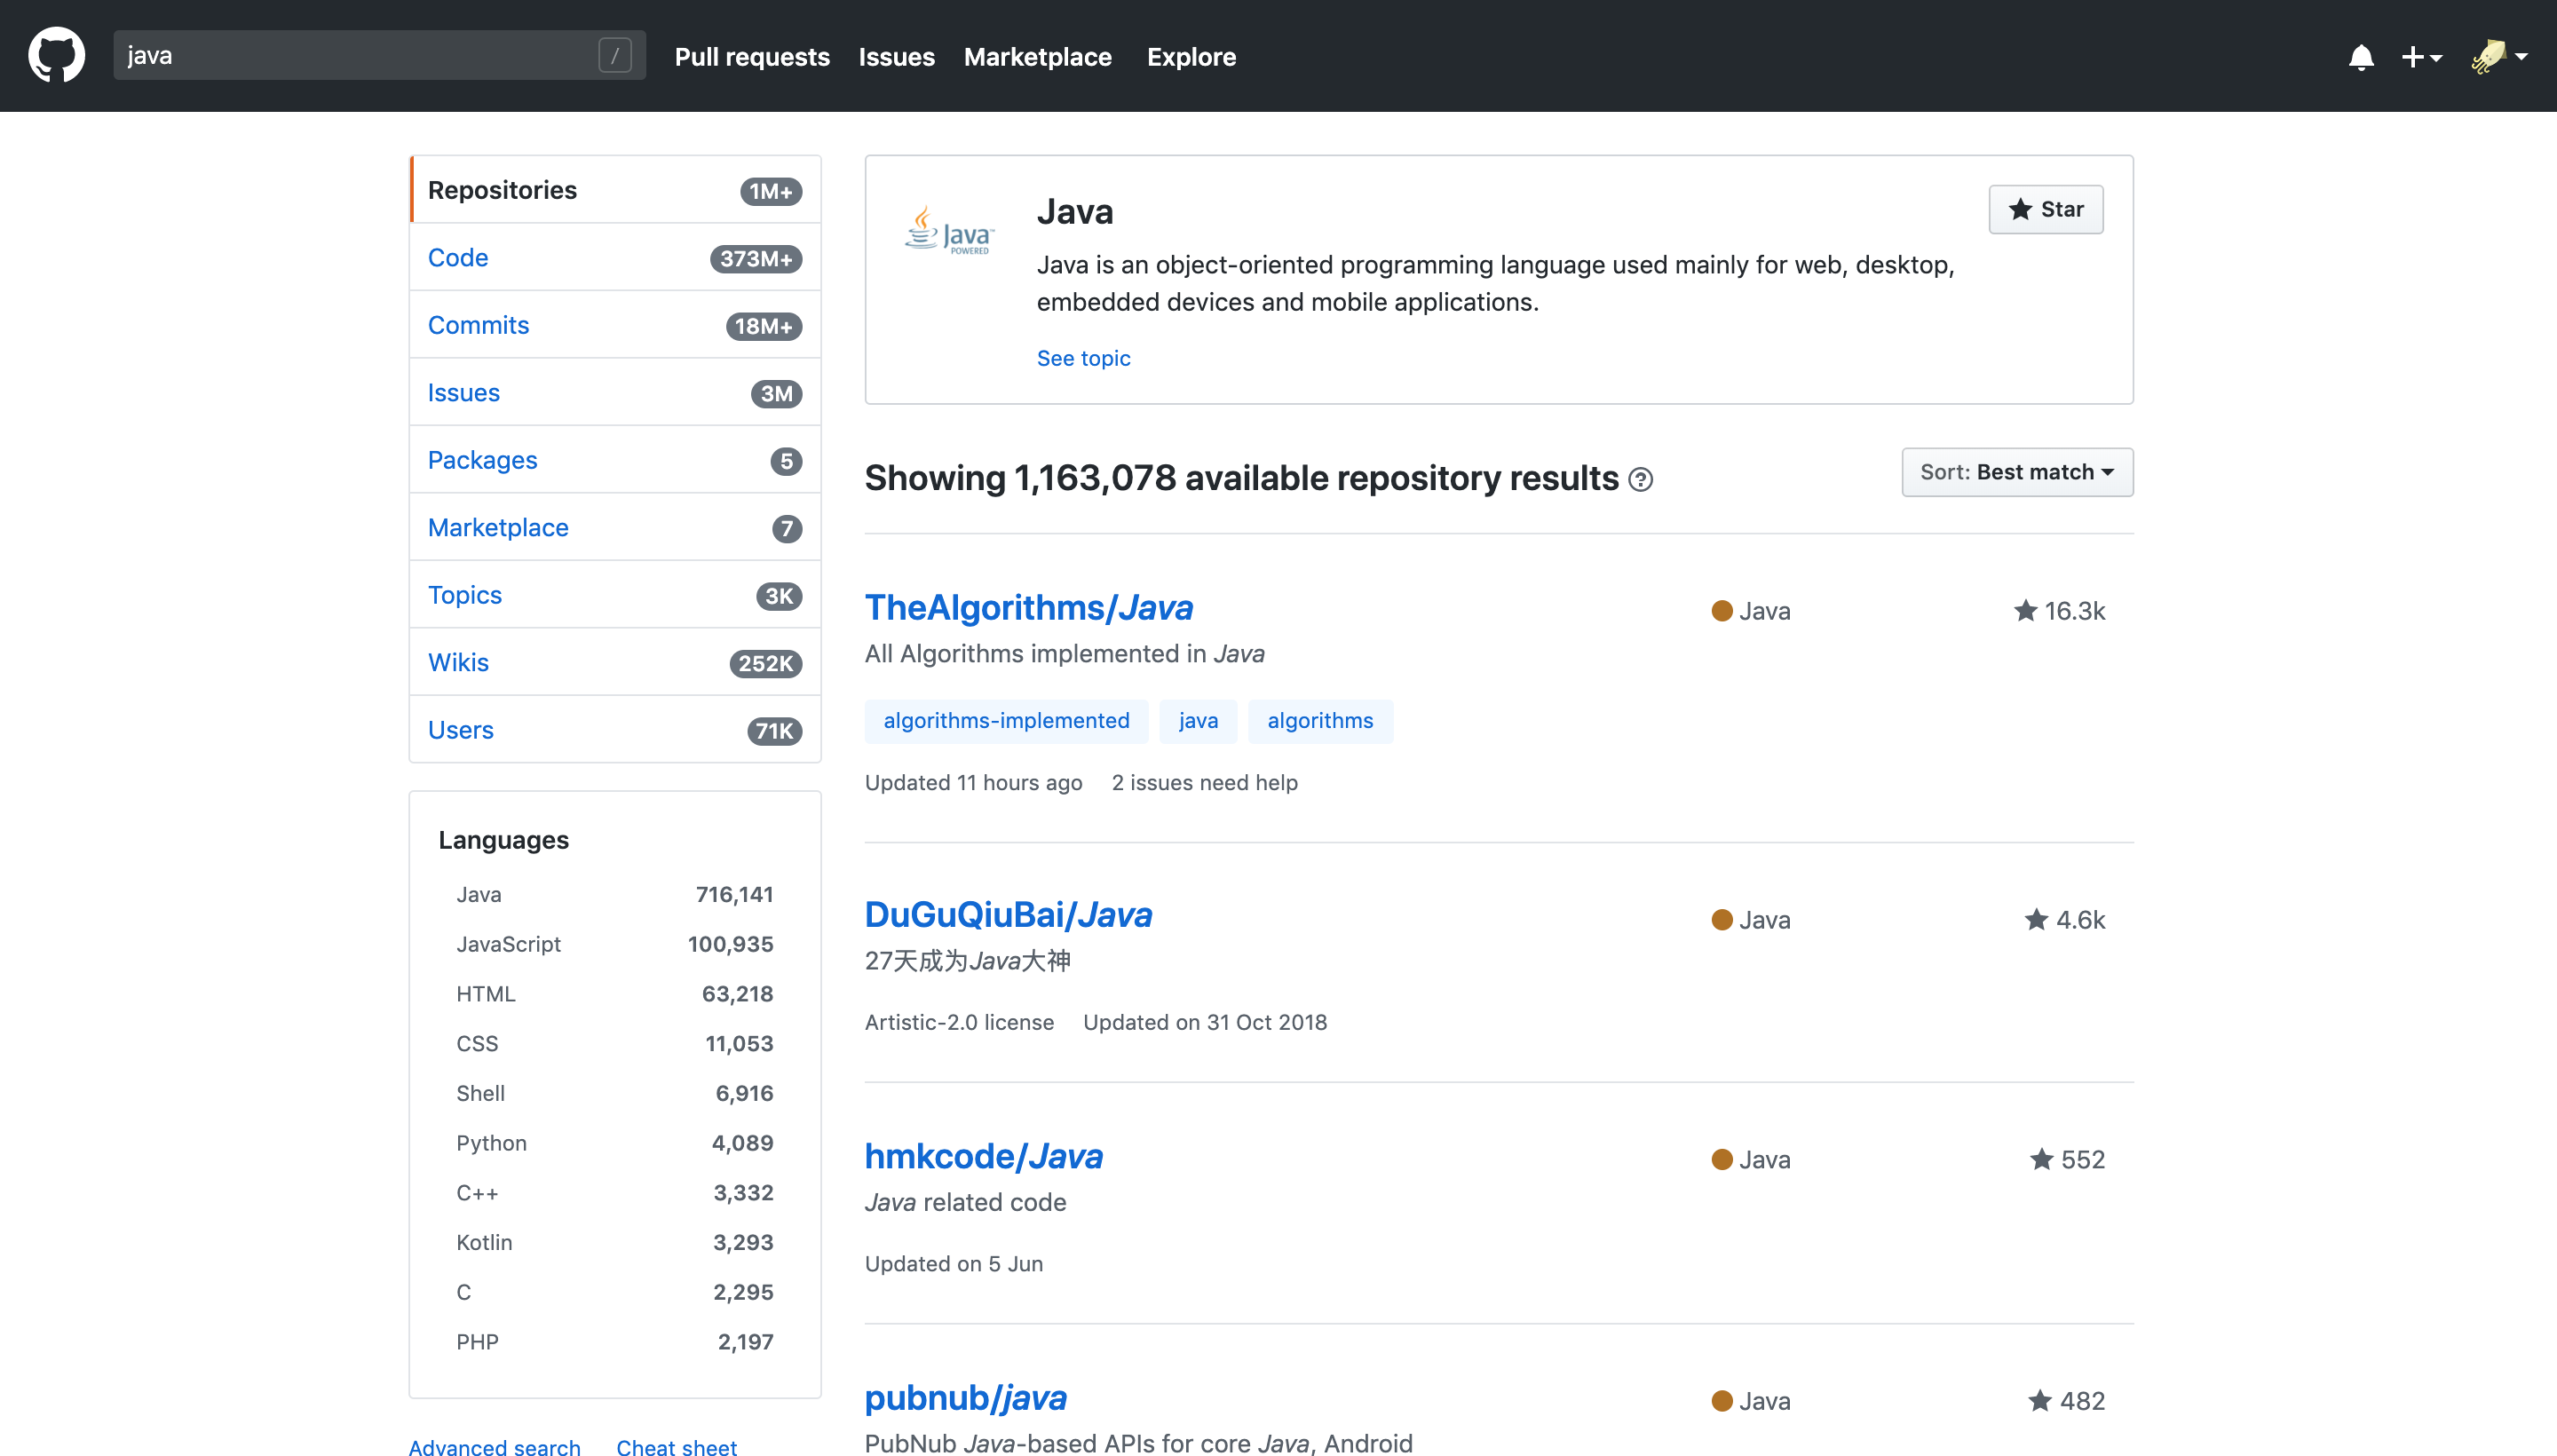
\includegraphics[scale=0.20]{./img/gh_os}
					\caption{Interface de github}					
				\end{figure}
			
				\subparagraph{Bitbucket\\}
				Très similaire à GitHub, Bitbucket est un hébergeur de code source ouvert qui permet à chacun de s’intéresser à des solutions open sources.

			\paragraph{Plateforme de promotion de projet}

				\subparagraph{Google Open Source\\}

				Avec plus de 2000 projets open sources sous sa tutelle, Google Open Source est un incubateur des nouveaux projets open sources sur le marché.
				La plateforme est simple, rechercher un projet comme une recherche google ou attendre la présentation de différents projets et laisser la magie opérer.

				\begin{figure}[!htb]
					\center
					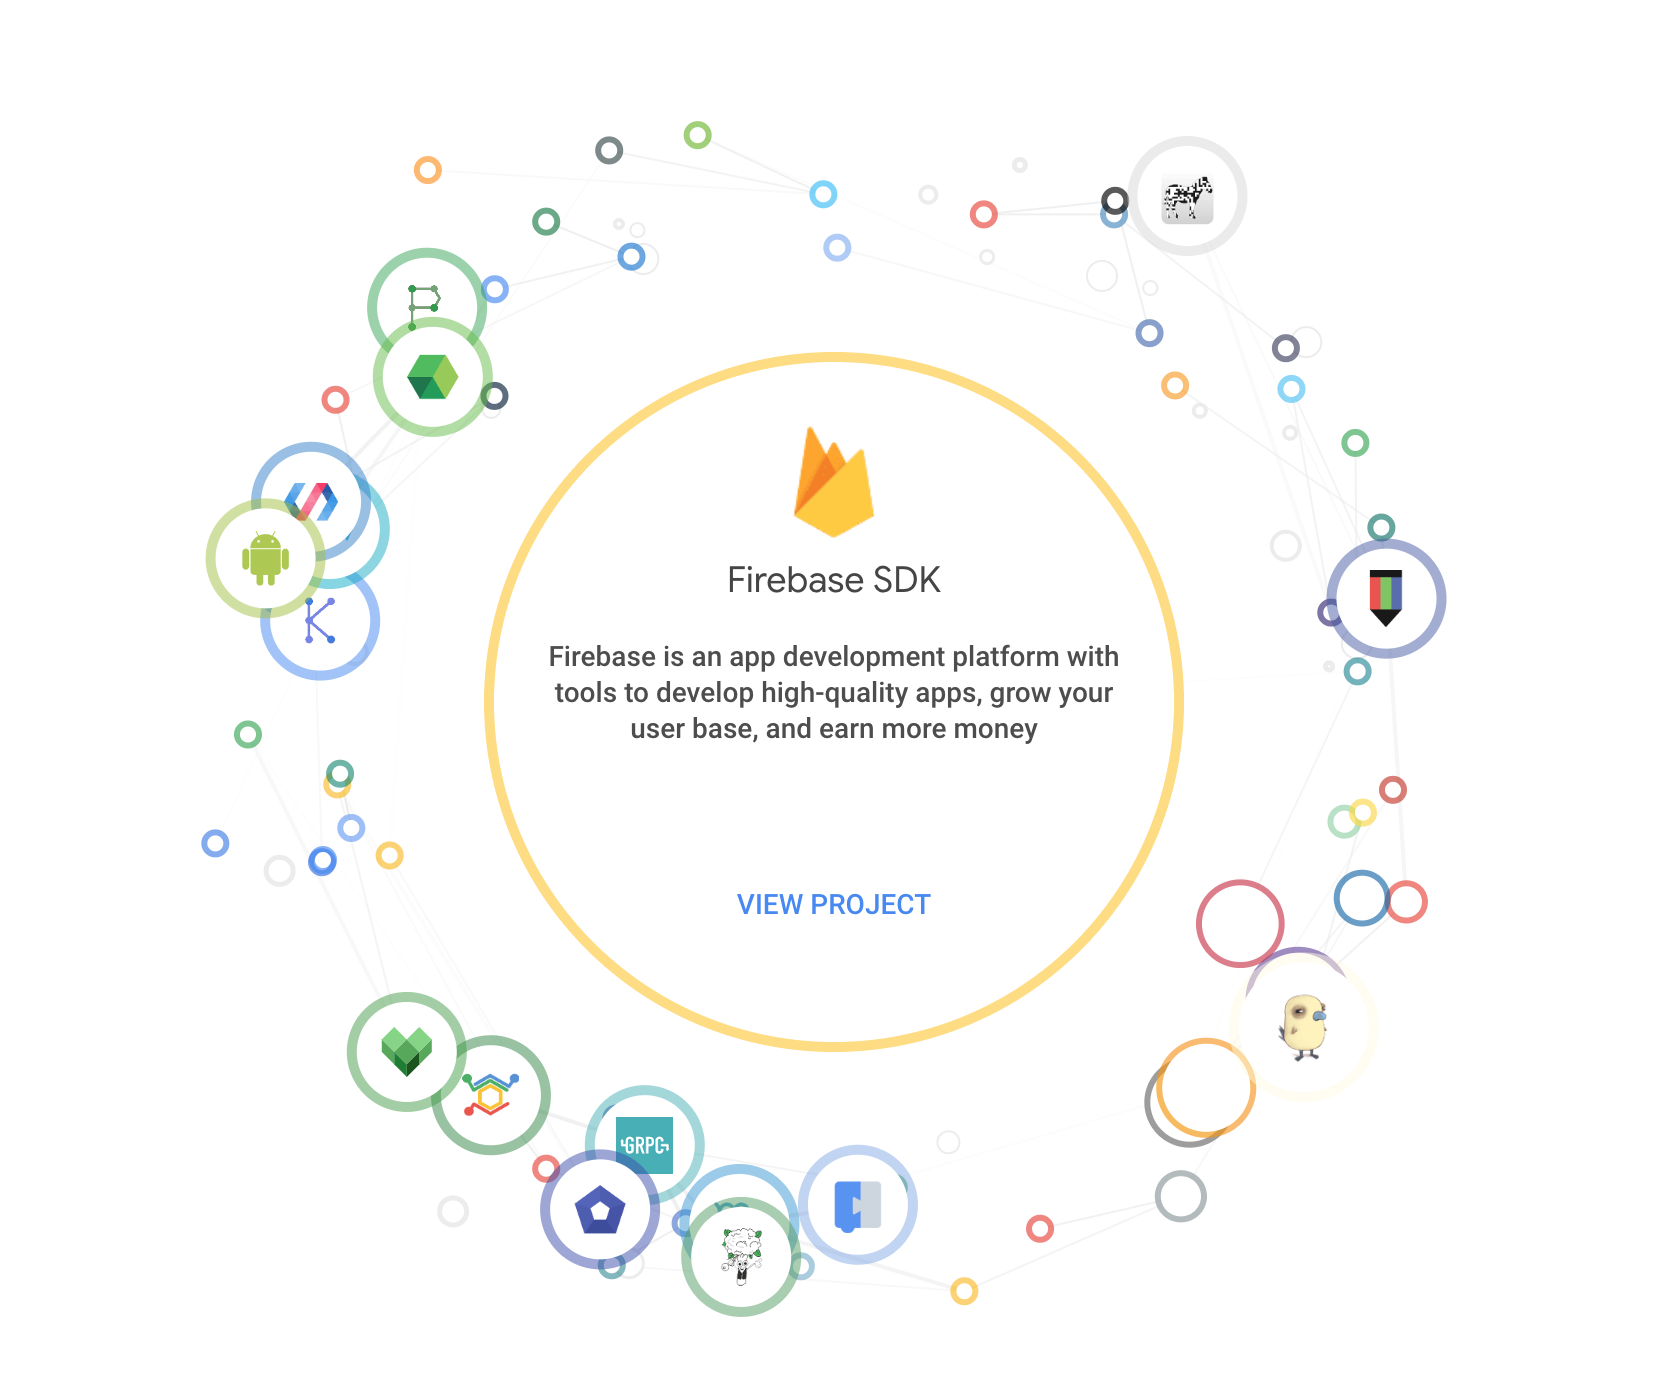
\includegraphics[scale=0.35]{./img/google_os}
					\caption{Interface de Google open source}					
				\end{figure}

				\newpage

				\subparagraph{Github Explore\\}
				L'interface simplifiée pour démarrer et trouver un projet open source auquel contribuer.

				\begin{figure}[!htb]
					\center
					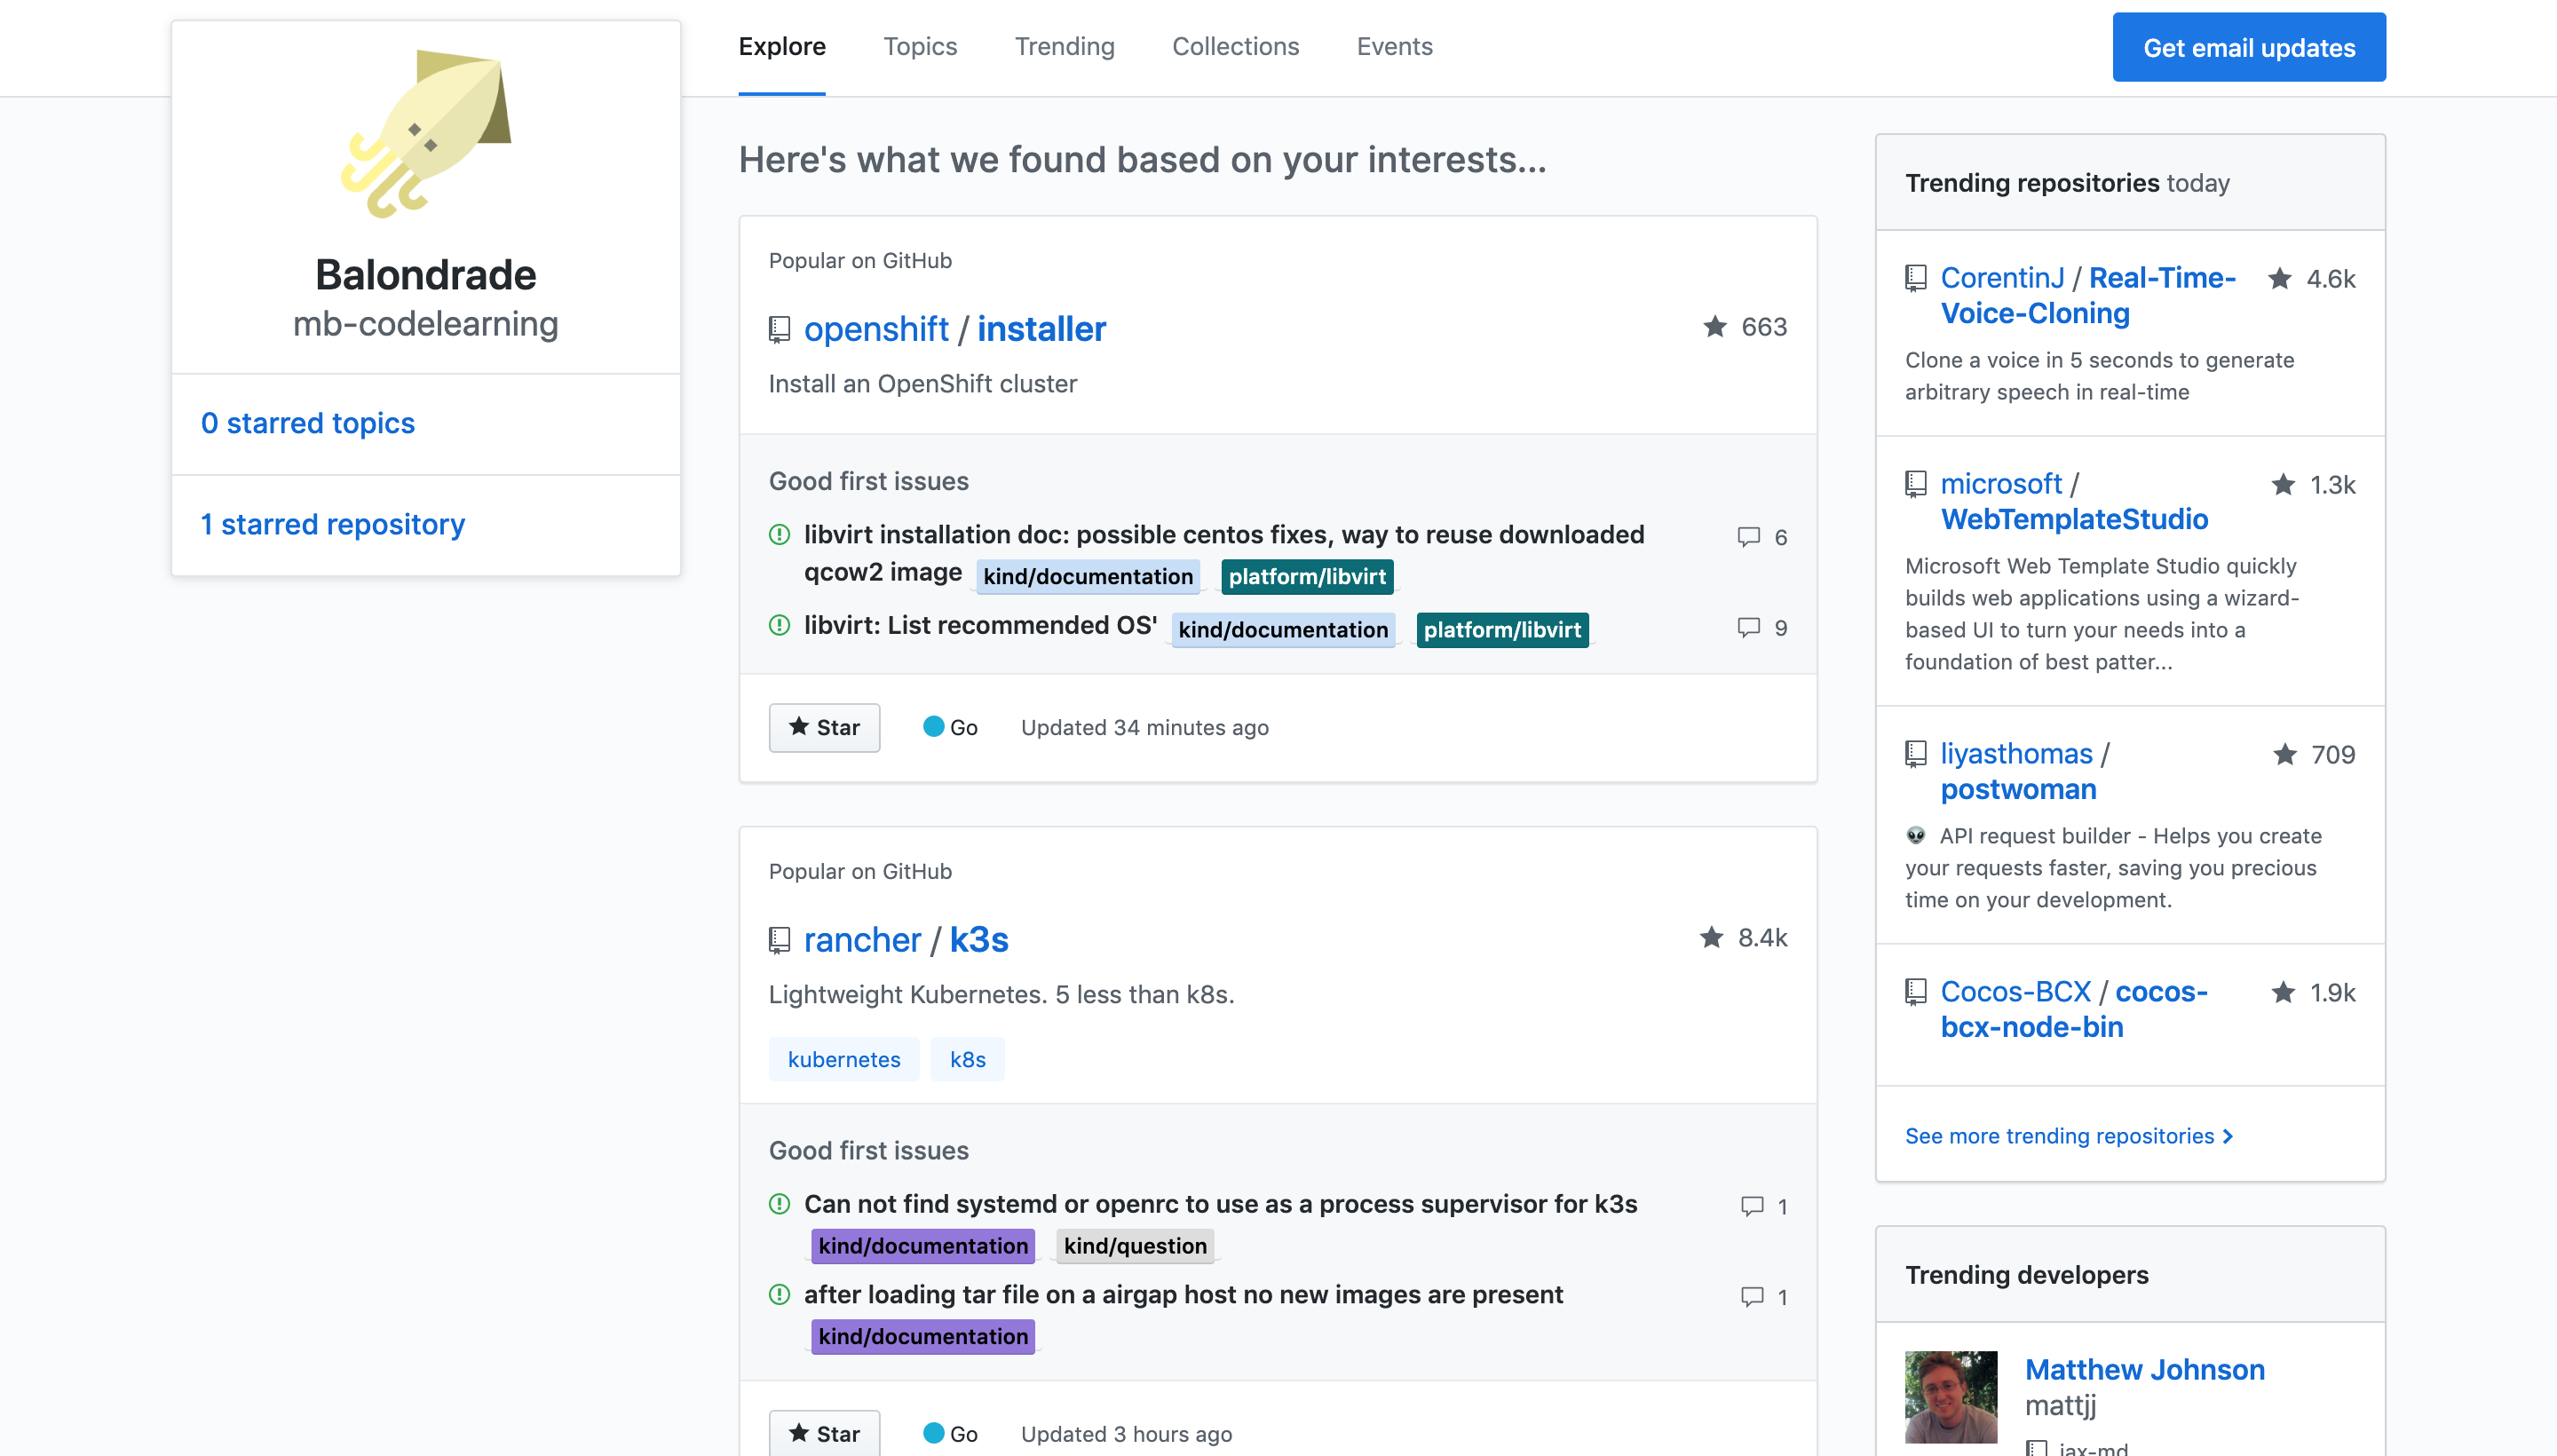
\includegraphics[scale=0.30]{./img/gh_explore_os}
					\caption{Interface de Github explore}					
				\end{figure}

				\subparagraph{Open source friday\\}
				Github propose comme date de rendez-vous tous les vendredis pour contribuer chaque semaines à enrichir le logiciel open source pour les curieux et les plus passionnés.

				\subparagraph{24 pull request\\}

				Chaque année pour la période de Noël, 24 Pull Request organise un moment de développement logiciel sur de l'open source avec comme objectif de remercier les éditeurs et leurs projets qui nous aident tant.
				En 2018, \textbf{1364} contributeurs ont participés sur \textbf{3321} différents projets open sources.

				\subparagraph{Code triage\\}

				La plateforme CodeTriage est non seulement utile pour trouver son projet et démarrer rapidement dessus mais nous envoit également un mail quotidien pour nous soutenir et nous rappeler nos engagements.

				\subparagraph{First Timers Only\\}

				On peut être pris au dépourvu lorsque l'on s'aperçoit que l'open source est un monde bien vaste que l'on ignorait. Pour cela, First Timers Only nous donne les clés pour débuter l'aventure en tant que contributeur.

				\subparagraph{Contributor ninja\\}

				Ici plus qu'un évenement c'est une plateforme avec une interface rapide, pour contribuer très rapidement à n'importe quel projet selon le langage de prédilection du contributeur potentiel.

				\begin{figure}[!htb]
					\center
					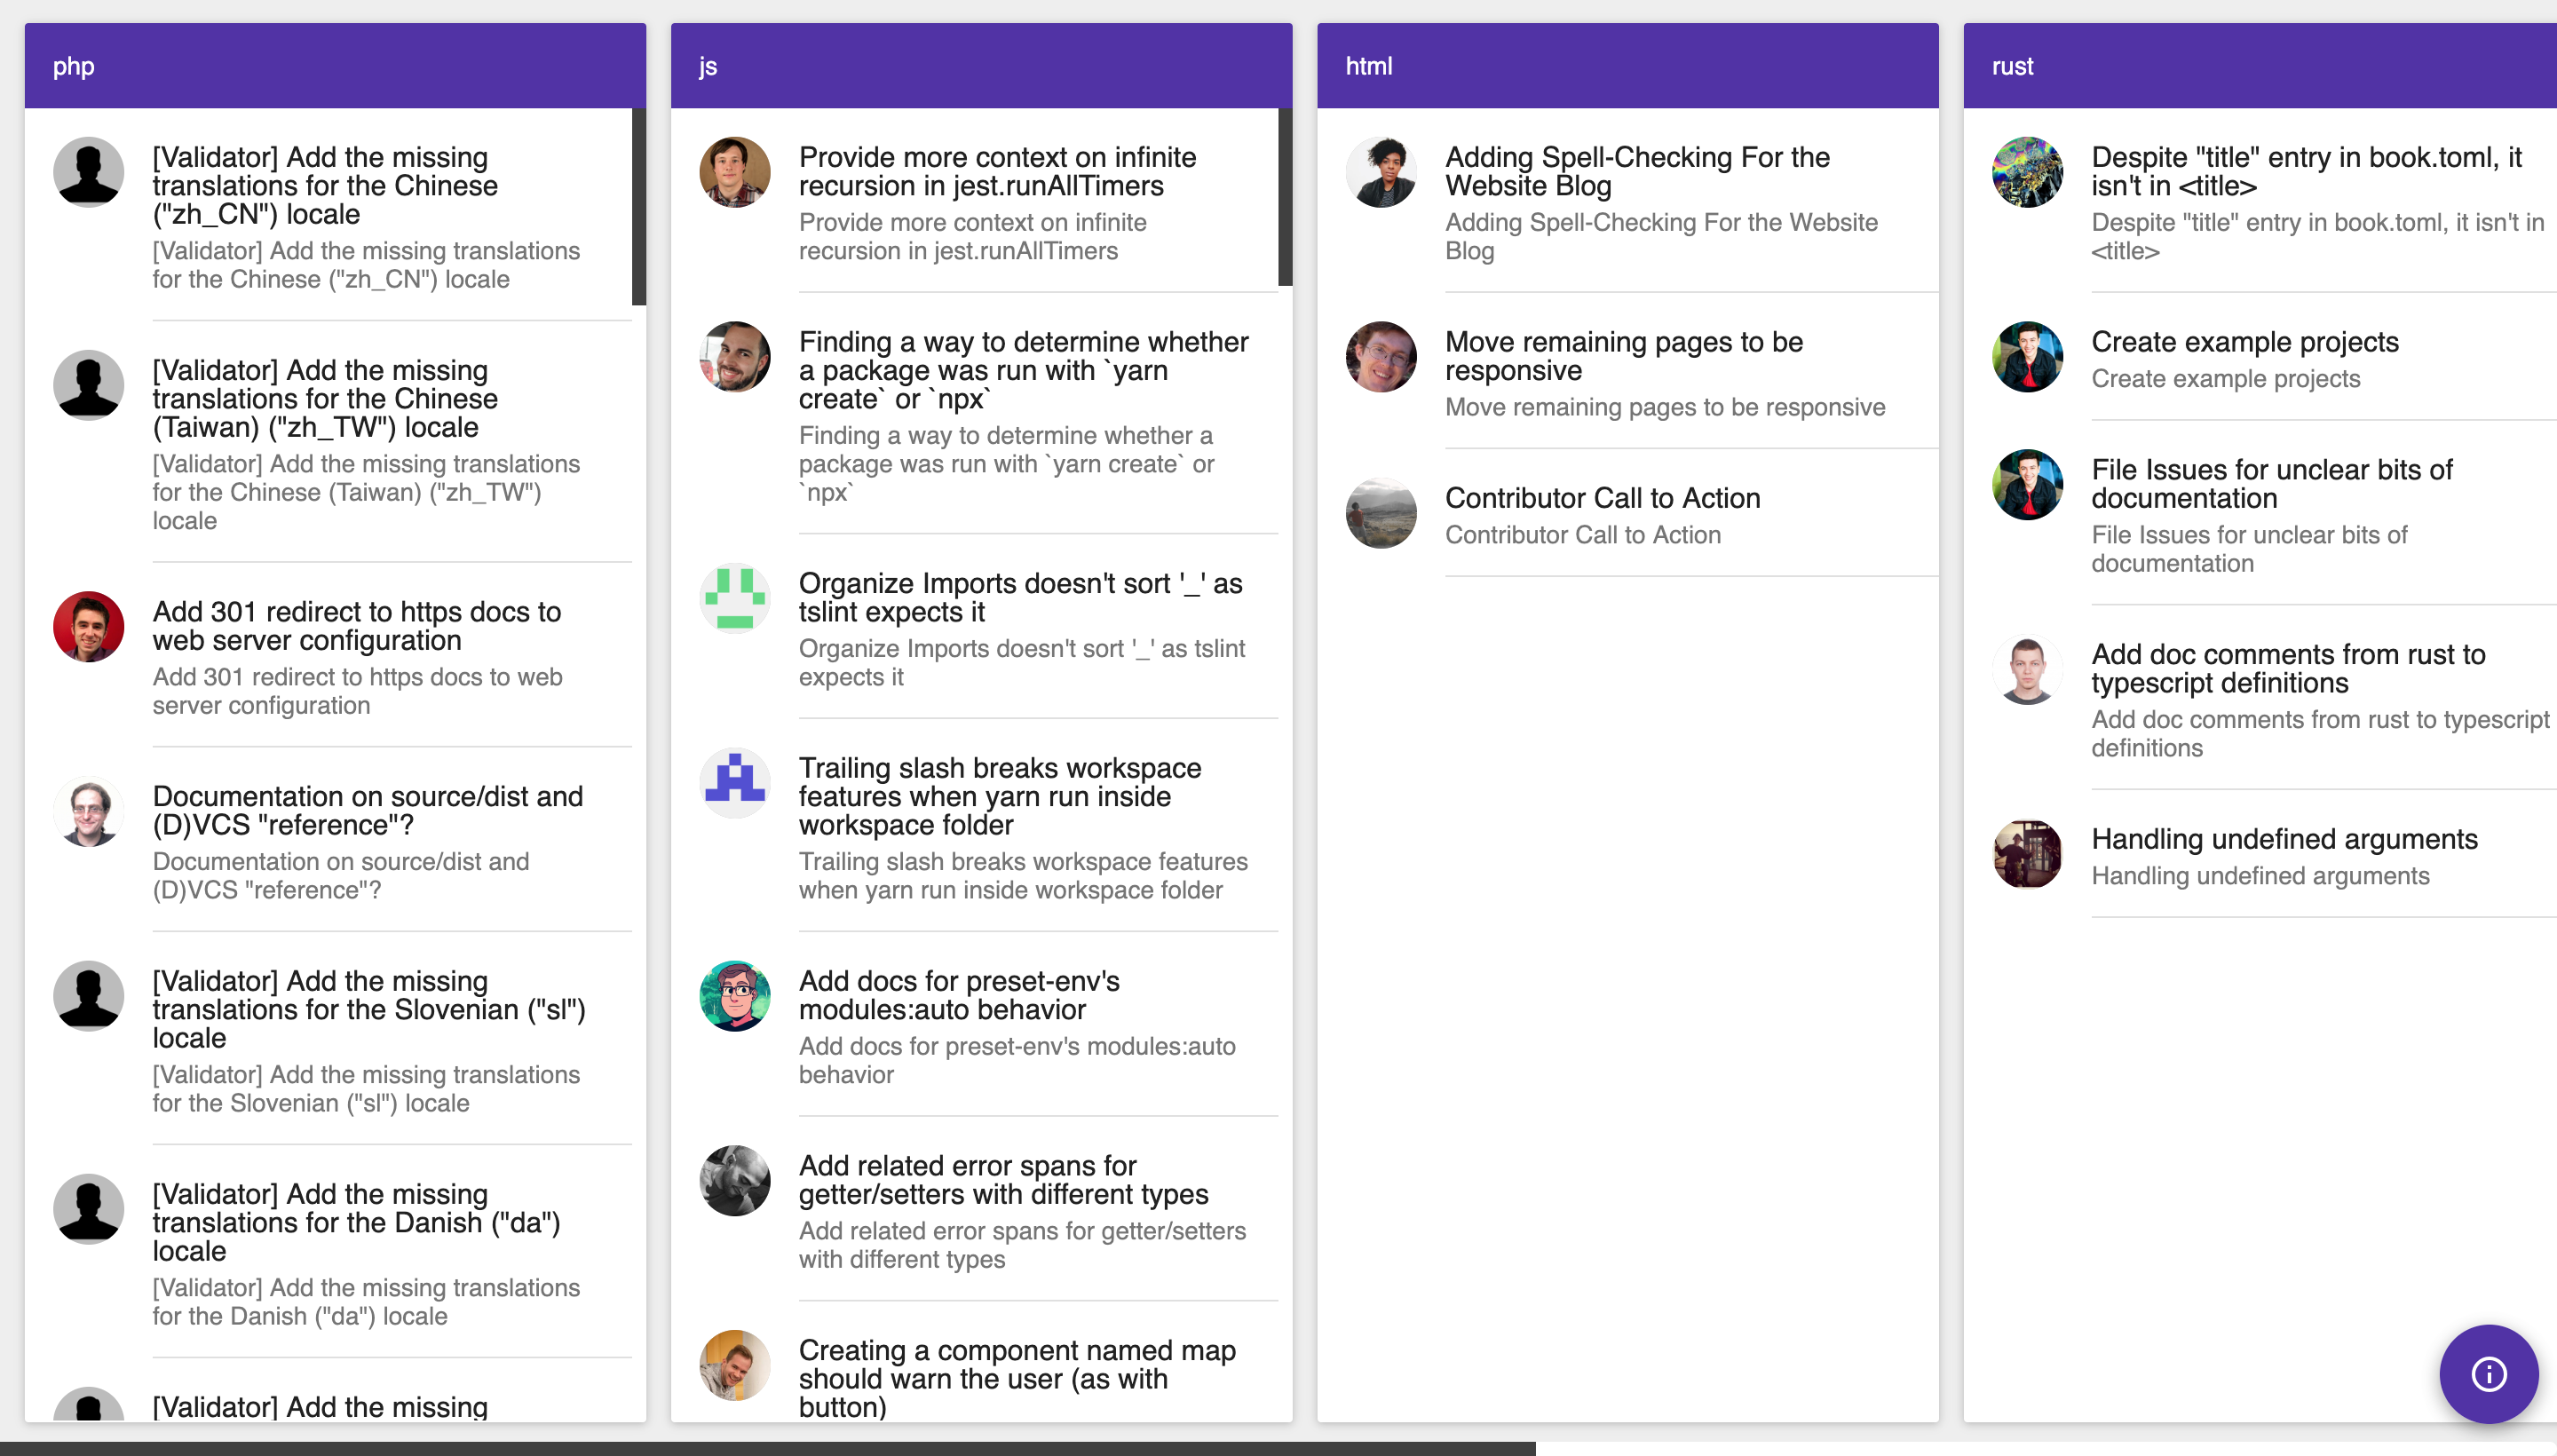
\includegraphics[scale=0.30]{./img/ninja_os}
					\caption{Interface de contributor ninja}					
				\end{figure}

				\subparagraph{Up for grabs\\}

				Pour vaincre toute forme de procrastination et la peur de faire le premier pas, up for grabs permet de rapidement trouver un projet et se lancer dans la contribution à l'open source. Le processus est simple :

				\begin{itemize}[label=\textbullet, font=\LARGE \color{burntorange}]
					\item Lire les quelques lignes du guide de contribution
					\item Installer le projet localement
					\item Laisser un message sur la tâche que l'on s'apprête à faire
					\item Se lançer dans le travail !
				\end{itemize}
		
		\paragraph{Pour conclure\\}

			L’open source est donc un mouvement important. Il apporte des valeurs de liberté, solidarité mais aussi des bénéfices tant pour les particuliers que pour les entreprises. 
		
	% --------------------------------------------------%
	%     												%
	%             Optimisation des ressources			%
	%       										    %
	% --------------------------------------------------%
	\section{Optimisation des ressources} 

		\paragraph{Concept de l'optimisation\\}

	 		Le succès d'un projet open source dépend du code mais aussi de sa communauté. Je cherche donc à optimiser les ressources humaines qui composent l'open source.

		\subsection{Le cerveau collectif}
			\paragraph{Introduction au cerveau collectif\\}

				A travers l'ouvrage de Napoleon \bsc{Hill}, intitulé \emph{« Réflechissez et devenez riche »}, on retrouve plusieurs fois la notion de cerveau collectif.

				L'élaboration d'un cerveau collectif constitue à regrouper des membres partageant les mêmes passions ou des intérêts complémentaires.
				Chaque personne veille à maintenir un climat de confiance.
				Au sein du cerveau collectif, l'intérêt est que chaque membre possède son domaine de connaissance particulier. 
				Napoleon \bsc{Hill} dans son oeuvre traite de personne instruite. Il définit une personne instruite, toute personne qui sans léser les intérêts d'autrui sait obtenir ce qu'elle veut.

				\subparagraph{Être instruit\\}

					Quand l'on sait que Henry \bsc{Ford} n'est allé à l'école que jusqu'à ses 6 ans. Malgré cela on peut qualifier cet homme d'instruit. Il fût traité de pacifiste ignorant pendant la première guerre mondiale par un journaliste. Afin de prouver son esprit inculte, les avocats des journalistes lui posèrent des questions innatendues sur des sujets variés. Face à tant de colles, celui-ci répondit:

					\begin{quote}
					« Permettez moi de vous rappeler que j'ai dans mon bureau une rangée de boutons électriques. Il me suffit d'appuyer sur l'un d'eux pour appeler un homme capable de répondre à n'importe quelle question relative à l'affaire dont je m'occupe personnellement(...), pourquoi je devrais avoir la cervelle farcie de culture générale alors que je suis entouré de collaborateur qui suppléent à toute lacune ou défaillance de ma part.»
					\end{quote}

			L'intérêt de vous partager cela est de vous faire réagir sur ce concept que l'on essaye tant d'inculquer à notre époque: la multi-compétence. A quoi bon souhaiter être bon dans une multitude de domaines, quand l'on peut être excellent voire une référance dans l'un des domaines qui nous siet tant.

			C'est sur ce principe que se base le fondement du cerveau collectif. \textbf{Utiliser le plein pouvoir de la connaissance de plusieurs individus} si compétents dans un domaine qu'il serait une perte de temps de chercher à les égaler.
			Egalement, je rajouterai que le cerveau collectif se veut complémentaire et que l'intéraction entre les divers membres permet d'aller encore plus loin ensemble mais surtout indépendemment.
			Ainsi, on peut définir un cerveau collectif par les concepts suivants : \\

			\begin{itemize}[label=\textbullet, font=\LARGE \color{burntorange}]
				\item Avoir un même idéal, but commun et être sur la même longueur d'onde.
				\item Un climat de confiance règne au sein de l'équipage.
				\item Chacun sa compétence qu'il améliore au fil du temps.
				\item Utiliser en collaboration les compétences de chaque membre dans leur domaine afin d'en résulter un plein pouvoir permettant de mener un projet à l'excellence.
			\end{itemize}

			\begin{quote}
			 « Si deux esprits travaillent ensemble, ils libèrent une troisième force invisible et intangible qui est semblable à un troisième esprit » - Napoleon \bsc{Hill} - \emph{Réflechissez et devenez riche}
			\end{quote}

			Imaginez si ce concept s'applique à l'ensemble de la communauté. C'est avec ce principe que nait mon idée d'optimiser la communauté d'un projet open source et le rendre incontournable.

			Le cerveau collectif à déja fait ses preuves pour nombres de personnes. Napoleon \bsc{Hill} décrit le succès du célèbre industriel Andrew \bsc{Carnegie} dont je vous invite à lire sa bibliographie. Il a utilisé le cerveau collectif avec son équipe d'une cinquantaine de personnes dans l'industrie de l'acier.

			\paragraph{Application du cerveau collectif au sein de la communauté\\}

			Bien évidemment avant de pouvoir appliquer ce concept il faut le faire accepter par les membres, qu'ils aient le même esprit de travail, ambition ou qu'ils puissent comprendre et se tourner vers ce mode de pensée.

				\subparagraph{Choisir les membres du cerveau collectif\\}

					Bien choisir son équipe est l'élement prédominant dans tout projet. Je pars du principe que l'on souhaite monter une communauté qui nous aidera à travailler sur notre projet. Il est primordial, avant de fonder le projet, de rechercher les membres essentiels qui composeront le cerveau collectif pour le mener à bien

					L'idée de démarrer dès que possible son projet est certe une direction tentante pour très vite faire contribuer des membres mais penser dès la conception du projet à monter le coeur du cerveau collectif permet de gagner un temps d'avance sur les étapes futures. Egalement cela renforcera les décisions prises afin que le projet se stabilise le plus rapidement possible.

					Alors avant de démarrer sur les chapeaux de roue, prenons le temps dès que l'on souhaite se lancer dans un projet, de trouver et d'impliquer les ressources humaines essentielles nécessaires à la construction de celui-ci. 

				\subparagraph{Choisir un support de communication adapté\\}

					L'outil de communication avec le cerveau collectif sera la principale source d'inspiration, de compte rendu, de retour et d'évolution du projet.
					Lorsque l'on souhaite se lancer en tant qu'éditeur d'un logiciel open source, il est important de veiller à mettre en place un outil de communication propre et clair sur lequel les décisions seront inscrites durablement.
					Savoir prendre des décisions précises sur lesquel nous ne revenons pas fait parti des qualités essentielles d'un dirigeant.

					Chaque membre du cerveau collectif est donc responsable des directions qu'il souhaite faire prendre au projet, à l'équipe, à la communauté et l'on attendra de lui une stabilité car il représente une partie importante du projet.

				\subparagraph{Gestion du cerveau collectif\\}

					Le cerveau collectif compose les membres au coeur du projet: le « noyau » mais aussi la communauté qui eux constituent les équipes qui gravitent autour du projet et réalisent les extensions.

					Gérer la communauté par domaine de connaissances ou métier permet de catégoriser et focaliser sur les contributions à apporter.
					Un cerveau collectif central et de multiple micro cerveaux collectifs autour permettront de maintenir le cadre d'évolution nécessaire à ce mode de pensée.

				\subparagraph{La communication au coeur de la stratégie\\}

					Et maintenant quoi ? On a un cerveau collectif, on a choisi les membres, on a respecté leur domaines de prédilection, mis en relation ... Mais où est la stratégie pour développer et déployer notre projet ?

					La gestion de projet inhérente à l'édition d'un logiciel est un standard que je ne développe pas ici (méthodologie Agile, gestion d'entreprise) mais on pourra compléter ceci avec l'ouvrage « Oser la confiance » comme nous le verrons dans la partie « Eveiller sa communauté » .

		\subsection{Rendre l'open source populaire}

			\paragraph{Pareto revisité\\}

				Une étude sur la participation de développeur et le code total rédigé rapporte que si l'on prend un projet avec 200 programmeurs participants, seulement 10 d'entre eux ont écris 50\% du code. C'est donc la preuve d'un investissement mal réparti généralement dans la programmation logicielle. Il faut donc veiller à \textbf{mettre en place une implication des participants au code} et plus largement au projet.

			\subsubsection{L'enseignement du logiciel open source}

				Comme mentionné dans l'introduction de ce document, le logiciel open source ne me semble pas suffisemment enseigné.\\

				\textbf{Qu'est-ce que j'entend par enseigner le logiciel open source ?}

				\paragraph{Susciter l'intérer de l'open source\\}

					Enseigner un logiciel open source par la mise en place d'efforts spécifiques à celui-ci. 

					Je retrouve dans le livre blanc «Point de vue sur l'open source » de Smile mon hypothèse concernant le manque d'enseignement de l'open source. Ce n'est pas en utilisant sans le savoir de l'open source ou en cherchant spécifiquement à remplacer tout logiciel propriétaire par du code ouvert que l'on enseigne l'open source. Il est nécessaire d'\textbf{expliquer les mécanismes} liés à l'open source, de prendre le temps d'\textbf{informer sur toute l'importance} de ce qui gravite autour de l'open source.\\
					Ceci afin de permettre à des centaines de programmeurs éparpillés sur la planète à coopérer de façon cohérente sur la réalisation des millions de lignes de code.\\

					Cela passe également, selon moi, par la \textbf{mise en relation des étudiants avec les communautés de développeurs}.

				\paragraph{Améliorer la recherche sur l'open source\\}

					Il est nécessaire d'encourager la recherche, comme le souligne Smile dans son livre blanc « Comprendre l'open source », qui se développe autour de ces logiciels et \textbf{fournir des outils nouveaux} pour accompagner leur essor.\\

					Les plateformes hébergeant l'open source sont à première vue trop réservées à la communauté de développeurs.

					Des spécificités métiers, comme dans le juridique et l'architecture logicielle pourraient se dégager afin de veiller au bon respect du code ouvert.

				\paragraph{Un gisement d'emplois futur\\}

					Tant par ses valeurs humanistes que par la contribution au patrimoine de l'humanité, l'open source doit être vue comme un bien commun qu'il faut cultiver ensemble.\\
					
					Tout autant que l'art qui est exposé dans de nombreux musées que l'on rend accessibles de temps en temps gratuitement pour contribuer à la culture de l'homme, \textbf{l'open source devrait être considéré de même}.\\

					Au cœur de l'activité industrielle, l'open source c'est 4,46 Md d'euros de \acrfull{ca} révèle l'enquête du \acrfull{cnll}, en 2017. 4 000 emplois nets ont été estimés d'ici 2020. La France est le leader Européen de l'open source, et pourtant, le système éducatif actuel ne perçoit pas ce gisement. 

		\subsection{Le modèle noyau-extension, tout un écosystème}
			
			 Dans ce schéma de développement connu pour déployer son activité open source, on distingue le noyau du produit sous la responsabilité de l'éditeur et les extensions réalisées par la communauté.

				Les principes de séparation sont les suivants:

				\begin{itemize}[label=\textbullet, font=\LARGE \color{burntorange}]
					\item Le noyau doit être d'une grande robustesse, il est certifié par l'éditeur, les contributions externes y sont rares
					\item L'interface entre le noyau et les extensions est bien documentée et stable, c'est à dire qu'un changement de version du noyau n'implique pas, du moins le plus souvent, un changement de version des extensions.	
					\item L'éditeur stimule la réalisation d'extensions, car elles donnent de la valeur à son produit et témoignent aussi de l'existence d'une communauté.
				\end{itemize}

				Ce \textbf{modèle noyau-extensions est celui qui réalise le meilleur point d'équilibre} entre les rôles respectifs de l'éditeur et de la communauté, réunissant la garantie et l'engagement de l'éditeur avec le dynamisme et l'énorme capacité de développement de la communauté.

				\begin{figure}[!htb]
					\center
					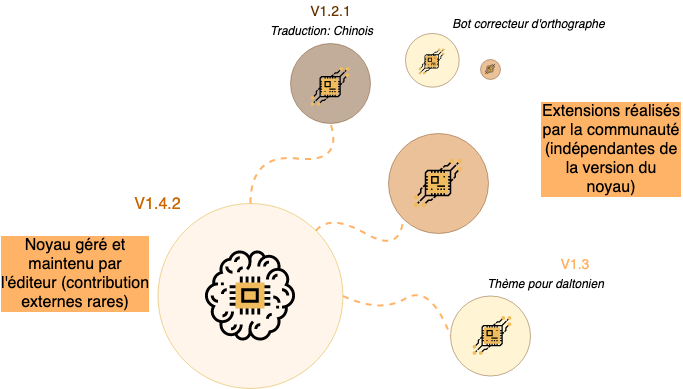
\includegraphics[scale=0.60]{./img/noyauextension_os.png}
					\caption{Représentation du modèle noyau/extension}					
				\end{figure}

				Ce modèle d'architecture présente plusieurs avantages:

				\begin{itemize}[label=\textbullet, font=\LARGE \color{burntorange}]
					\item Ne pas faire grossir inutilement un programme en se concentrant sur l'essentiel du business et de sa fonctionnalité.
					\item Jouer sur l'aspect modulable et simple du logiciel et concurrencer les logiciels propriétaires qui, sous pression, rajoutent de plus en plus de fonctionnalités sur leur logiciel jusqu'à le rendre trop lourd.
					\item Déjouer la concurrence sur le marché, car la communauté se concentre sur la création et l'amélioration perpetuelle des extensions.
					\item Éviter de destabiliser son logiciel, car les fonctionnalités peuvent être ajoutées sous forme de modules.
				\end{itemize}

				Le modèle noyau-extension permet de tracer cette frontière entre l'éditeur et la communauté tout en s'assurant que la communauté trouve sa place au sein du produit et que chacun puisse répondre à son besoin.

				Pour favoriser la mise en place et le maintien du modèle noyau-extension, l'éditeur peut \textbf{mettre généralement en place une plateforme pour accueillir ces extensions} afin d'avoir une meilleure visibilité, classer par popularité, trier selon les besoins et de rendre gloire aux auteurs de ces extensions.
			
		\subsection{Eveiller sa communauté}

			Afin de faire naître et grandir sa propre communauté autour de son produit open source, il existe déjà quelques points clé soulignés dans le livre blanc « Comprendre l'open source » de Smile:

			\begin{itemize}[label=\textbullet, font=\LARGE \color{burntorange}]
				\item Semer la graine en mettant en ligne son code source. Être patient vis-à-vis de l'épanouissement de la communauté qui va prendre racine.
				\item Être transparent tant dans son projet et ses orientations que dans la gouvernance du projet.
				\item Choisir et décréter son support d'échange avec la communauté afin de centraliser la communauté sur ses outils.
				\item Instaurer sa politique de l'open source en proposant un modèle noyau-extension, celui qui fonctionne pour le mieux. Bien préciser quels sont les aspects que l'on veut retrouver dans notre vision open source.
				\item Inspirer des valeurs : le logiciel que l'on va construire n'a pas de but lucratif ou du moins, il est moindre. Ceci aide à construire la communauté plus facilement, car elle n'aura pas l'idée qu'on génère de l'argent sur son dos. On aspire à aider, changer le monde. Il faudra trouver l'idée d'une mission que les gens adoptent.
			\end{itemize}

			Le respect de ces standards permet d'instaurer la communauté au projet. Pour compléter ces bonnes pratiques, j'y ajoute la notion de gestion de la communauté en m'appuyant par les propos tirés du livre « Oser la confiance » qui sont les suivants :

			\paragraph{Les valeurs\\}

			La mission que doit relever l'éditeur à travers son projet open source n'est pas anodine. Les valeurs incarnée par celle-ci permettent d'attirer le contributeur. Je souhaite donc \textbf{les mettre en avant dans la partie présentation des projets}.

			Dans l'ouvrage « Osez la confiance », une entreprise de construction navale est sur la faillite, le nouveau PDG, Bertrand \bsc{Martin} ne leur indique pas de solution concrète, pour autant, le personnel à su relever la pente. 
			\begin{quote}
			\emph{« C'est parce que le personnel le voulait, qu'il avait pu s'approprier le projet, qu'il en comprenait les enjeux, que nous avons opéré avec le maximum d'efficacité »}
			\end{quote}

			\paragraph{Mettre en confiance\\}

			Vincent \bsc{Lenhardt} dans son livre nous confie le vrai pouvoir de la confiance, il emploie le mot \emph{empowered} qui définit clairement que lorsque l'on attribue toute confiance, toutes ressources et l'aide nécessaire à l'acteur d'un projet, celui-ci donne le meilleur de lui même.

			Il y a donc une attitude à rechercher chez l'éditeur, c'est la confiance en ses contributeurs. \textbf{Apprendre à faire confiance en sa communauté} en leur confiant des tâches essentielles, avec des enjeux dont ils ont pleinement conscience permet de dépasser ses limites pour atteindre les sommets.

			C'est ce qui a permis de relever l'entreprise de chantier naval de Bertrand \bsc{Martin}.

			\paragraph{Donner l'exemple\\}

			L'éditeur se doit de faire partie des contributeurs, se mettre non au-dessus, mais dans le bocal permet à chacun de se responsabiliser et comprendre que l'on est une force selon le dicton « L'union fait la force ». Dans « Oser la confiance », ce principe est bien détaillé. Vincent \bsc{Lenhardt}, analyse cela en concluant que le pouvoir et l'initiative seront entre les mains des acteurs ce qui les pousseront à mettre en oeuvre les décisions. On ne recherche plus forcément la compétence de l'éditeur, ni de donner les solutions, mais de \textbf{déléguer et faire partie du groupe} afin d'améliorer la responsabilité des acteurs.

	% --------------------------------------------------%
	%     												%
	%              Etude du consommateur				%
	%       										    %
	% --------------------------------------------------%
	\section{Etude du consommateur} % in progress

		\subsection{Le choix du consommateur}

			\paragraph{L'activité d'un projet\\}

			Afin d'établir un choix de solutions pérennes, le consommateur va s'interroger sur l'historique du projet et les orientations de celui-ci s'il provient d'un « \gls{fork} » ou si un fork est fortement probable comme le souligne la société OpenDsi dans son article de blog intitulé « Comment choisir un logiciel libre ou open source ».
			Il pourra alors s'orienter vers toutes sources d'informations disponibles : blog, article, forum de discussion et liste de diffusion des activités lié à ce projet. Il peut être également intéressant de faire attention au nombre de contributeurs au projet, car il peut y avoir certaines incohérences autour d'un projet massivement adopté et le nombre de développeurs qui le portent.

			\paragraph{La nature des contributions\\}
			
				Dans certains domaines, notamment dans celui de l'industrie, un projet open source peut fortement dépendre des contributions d'une entreprise et non d'une communauté. Ceci peut prendre différentes tournures, le projet peut partir vers un modèle propriétaire au bout d'un certain temps. Prendre des décisions qui arrangent l'entreprise en question et qui sera pénalisant pour l'utilisateur final.

				Ainsi, le consommateur sera davantage \textbf{rassuré par le nombre de contributeurs et la diversité de ceux-ci}, signe d'indépendance et de pérennité du projet.

			\paragraph{Les droits inhérents de la licence\\}

			En fonction du besoin du consommateur comme je vous l'ai présenté à plusieurs reprises, les licences vont permettrent la ré-utilisation, la commercialisation et bien d'autres actions au projet. Le choix d'un logiciel open source se fait donc également entre la \textbf{cohérence du besoin et des idées du consommateur et les permissions accordées} à celui-ci.

		\subsection{L'expérience des consommateurs}

			Github a lancé une étude auprès de nombreux dépôts de code et de la communauté qui gravite autour. C'est plus de 3 800 projets open source et plus de 500 réponses qu'ils ont réussis à obtenir les conclusions suivantes:

			\paragraph{Le retour des consommateurs \\}

				Beaucoup de critiques comme les propositions de corrections ou d'améliorations sont des retours appréciables du consommateur. C'est ce que souligne l'article « Les logiciels libres meurent lentement sans contributions » de Framasoft, une société éditrice de solutions libres.
				Cette contribution permet aux éditeurs de progresser et de s'adapter au marché et à la demande.
				Ainsi, il s'agit d'une notion à prendre en compte dans l'optimisation de la communication avec les consommateurs. Il est possible \textbf{d'intégrer un module sur la plateforme de promotion qui facilitera les retours d'informations et critiques à l'éditeur}.

			\paragraph{Les problèmes rencontrés par les consommateurs\\}

				Les consommateurs recensent de nombreux problèmes que l'on retrouve dans l'open source et qui peuvent être un frein à son utilisation. Lors d'une étude réalisée par Github, il ressort que la documentation et le support sont essentiels auprès des consommateurs auquel je suggère de faire principalement attention.

				\begin{figure}[!htb]
					\center
					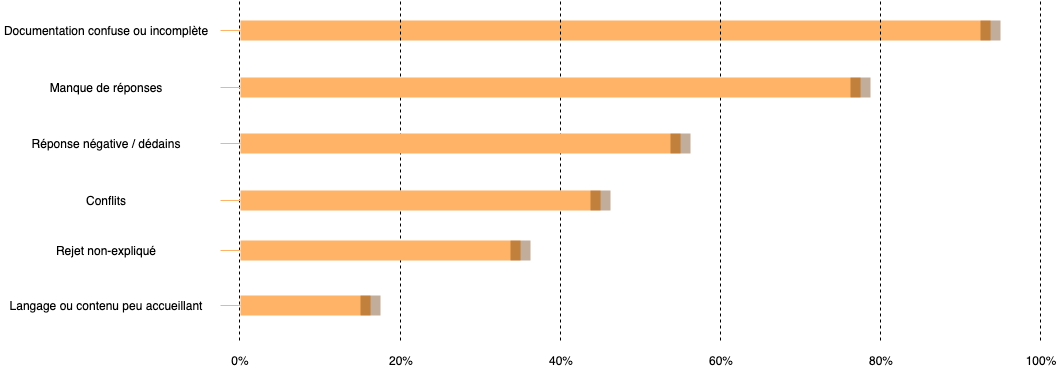
\includegraphics[scale=0.50]{./img/pb_os.png}
					\caption{Problèmes rencontrés dans l'open source par les utilisateurs}
   					\caption*{\color{silver}Source: opensourcesurvey.org}
				\end{figure}
				

			\paragraph{Un climat néfaste ?\\}

				Au sein de projet open source due au fait d'une communauté décentralisée, virtuelle et des enjeux, nous pouvons retrouver de nombreuses violences dans les communications entres les consommateurs et les éditeurs. Le \textbf{respect dans la communication et la bienveillance} sont des facteurs essentiels pour la satisfaction client et donc croître le nombre d'utilisateurs.

				\begin{figure}[!htb]
					\center
					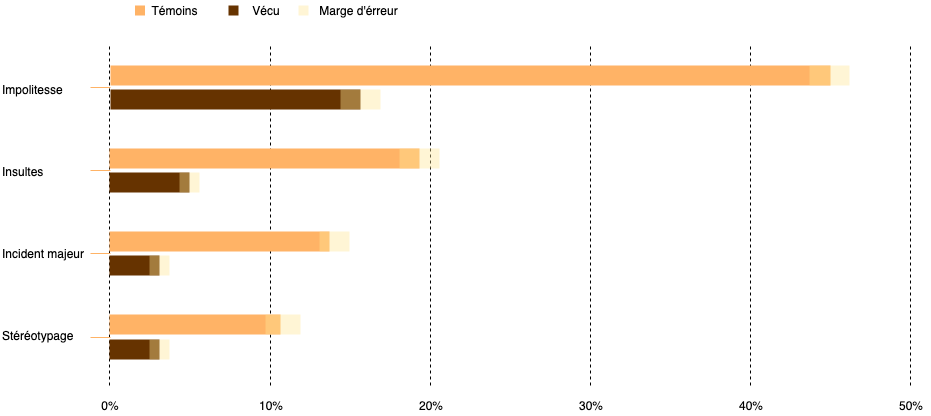
\includegraphics[scale=0.50]{./img/ng_behaviour_os.png}
					\caption{Comportements néfastes dans l'open source}
   					\caption*{\color{silver}Source: opensourcesurvey.org}
				\end{figure}

			\paragraph{Ce qui est regardé dans le choix d'un logiciel open source\\}

				 Sur les utilisateurs interrogés, un classement des critères de sélection d'une application a été réalisé. Les premiers regards des consommateurs sont portés sur la stabilité et la sécurité du projet open source. Je préconise ainsi l'\textbf{utilisation d'outils spécialisés pour vérifier, certifier le projet} open source pour rassurer les consommateurs.

				\begin{figure}[!htb]
					\center
					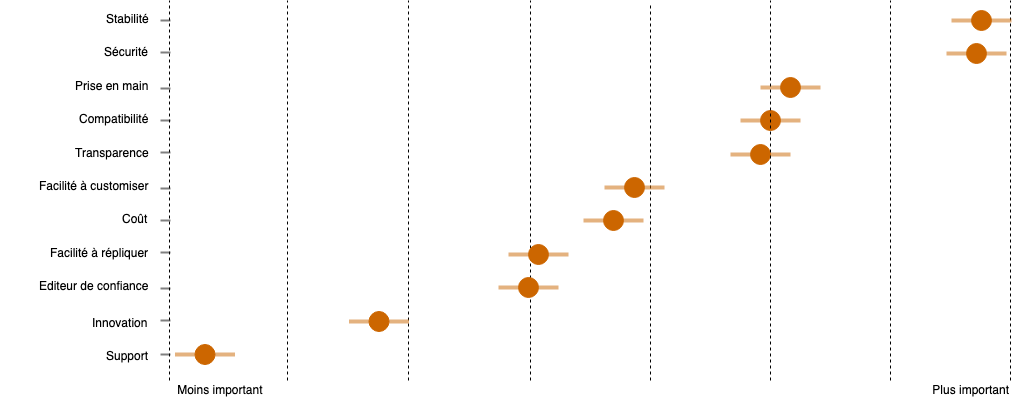
\includegraphics[scale=0.50]{./img/value_soft_os.png}
					\caption{Ce que les utilisateurs d'open source recherchent dans les logiciels}
   					\caption*{\color{silver}Source: opensourcesurvey.org}
				\end{figure}


	% --------------------------------------------------%
	%     												%
	%            Le marché de l'open source			    %
	%       										    %
	% --------------------------------------------------%

	\section{Le marché de l'open source} % in progress

		\paragraph{Libre n'est pas gratuit \\} 

			C'est bien l'un des principes de l'open source: même si l'on a pour vocation de s'étendre et de distribuer son produit, il est nécessaire, si ce n'est vital pour certains éditeurs de trouver une source de revenus pour leur logiciel.\\
			Il faut savoir qu'il existe une différence entre faire payer un logiciel propriétaire et un logiciel open source. 
			\begin{description}[font=\color{burntorange}]
				\item [Payer un logiciel propriétaire : ] permet non seulement d'apporter des revenus à une entreprise, mais d'obtenir un « droit de possession », d'acquisition du logiciel.
				\item [Payer un logiciel open source : ] n'est pas un prix d'acquisition ni un droit d'utilisation mais une source de revenus à l'éditeur pour permettre au logiciel de prospérer.
			\end{description}

		\subsection{Les acteurs de l'open source}
			Il existe dans l'open source 4 grands acteurs:

			\begin{description}[font=\color{burntorange}]
				\item[Les fondations:] telles qu'Apache ou Eclipse, sont des organismes à but non-lucratif qui stimulent et pilotent le développement de grands produits open source.
				\item[Les distributeurs:] Redhat, Canonical (Ubuntu) ou Mandriva sont des distributeurs (très souvent éditeurs par la même occasion). Ils sélectionnent des outils et composants autour d'un noyau Linux, en assurent le packaging, la distribution et le support.
				\item[Les éditeurs:] diffusent des logiciels sous licence open source, ils réalisent la promotion de leurs produits et proposent du support
				\item[Les prestataires : ] vendent des services sur l'open source. Il peut s'agir de conseils, d'intégrations, de support, de la formation, des solutions d'hébergement, etc.
			\end{description}

			Je m'intéresse particulièrement aux éditeurs de l'open source qui devront mettre en place des solutions assurant la stabilité financière de leur activité.\\

			 Les éditeurs de l'open source sont en recherche de prospérité, car pour les autres acteurs, la taille, la mission et le produit présenté ne pose plus aucune difficulté de revenu. Doit-on encore se soucier du bon développement de Linux et de sa communauté ? Ces géants de l'open source, ont des moyens marketings (plus de 60\% de leurs revenus) et financiers bien supérieurs aux éditeurs et prestataires qui restent pour la majorité des petites et moyennes entreprises.

			\emph{Comment fonctionne donc le modèle économique ou « business model » de ces entreprises ?}\\

		\subsection{Chez les éditeurs}

			Même s'ils bénéficient de l'open source pour réduire le coût de leurs ressources, celles-ci ne comblent pas les besoins de financement de la partie développement en interne, de l'hébergement et du marketing. Il est donc nécessaire de trouver des sources de revenus pour les éditeurs.

			Parmis celles-ci, on distingue 3 principales sources pour l'éditeur:

			\begin{itemize}[label=\textbullet, font=\LARGE \color{burntorange}]
				\item Vendre des licences
				\item Vendre du support
				\item Vendre de l'intégration
			\end{itemize}

			\subsubsection{Vendre des licences}

				Même s'il est interdit de faire payer l'utilisation d'un logiciel open source, les éditeurs ont bien compris commment faire bon usage de la « double licence ».

				\paragraph{Double licence commerciale\\}

					Il est possible de distribuer une œuvre dérivée utilisant le programme sans diffuser ses sources à l'aide d'une licence commerciale.\\
					Le programme officiel open source est gratuit mais sa version dérivée elle est payante à travers l'achat d'une licence commerciale.\\
					Pour l'entreprise MySql par exemple, la vente de licence représente plus de la moitié du \acrfull{ca}.

				\paragraph{Les extensions payantes\\}

					L'éditeur peut proposer des extensions aux fonctionnalités présente dans le logiciel open source. Le logiciel initial est suffisemment de qualité et donne envie de payer quelques extensions \textit{optionnelles} supplémentaires pour le confort et le besoin de l'utilisateur.

				\paragraph{Un support uniquement sur licence commerciale\\}

					Ici aussi, le logiciel est sous licence open source mais si l'on désire avoir le moindre support dessus, il faudra se tourner vers son confrère et sa licence commerciale.

			\subsubsection{Vendre du support}

				La prestation de support est une source principale de revenu pour l'éditeur, même s'il doit pour cela faire face à la concurrence potentielle de prestataires tiers que je précise juste après.

				Le support d'un logiciel inclut généralement :

				\begin{itemize}[label=\textbullet, font=\LARGE \color{burntorange}]
					\item L'accès privilégié aux correctifs et ressources spécifiques
					\item Une prise en chage des problèmes (anomalies, utilisation, mise en oeuvre ...)
					\item Des prestations d'audits, de certifications, ou de prises de contrôle à distance, ainsi que la surveillance proactive et les corrections.
				\end{itemize}

				On peut distinguer différents modèles de financement concernant la vente de support.

				\paragraph{Uniquement le support\\}

					Certains éditeurs misent uniquement sur la vente de support. Le logiciel est gratuit mais le support lui est payant. Ce modèle de financement fonctionne pour certaines entreprises comme Tiny(OpenERP), Nuxeo.\\

					Le problème est qu'en cas où le support n'a pas été utile l'année souscrite pour cause de stabilité du logiciel, le client voudra surement le résilier pour la suite.\\

					Plus le produit est de qualité, moins le support est facile à vendre car le client rencontre moins de difficultés.\\

					L'avantage est que plus on avance dans la technologie et plus la concurrence est présente on doit donc sortir des nouveautés constamment ce qui fragilise le produit et le rend instable. Le support est donc précieux dans le cadre professionnel.

				\paragraph{Faire payer la stabilité\\}

					Pour d'autre éditeurs, la stabilité d'un logiciel peut devenir source de profit. L'idée est de proposer deux logiciels:\\

					\begin{itemize}[label=\textbullet, font=\LARGE \color{burntorange}]
						\item Celui en licence open source sera classifié de « community edition ». Il sera présenté comme instable, pas entièrement testé, à ne pas déployer en production.
						\item Tandis que le logiciel sous licence non-libre sera la licence sécurisée, une version « enterprise-ready », « fully tested ».
					\end{itemize} 

					Au final, la version community, c'est celle en cours de développement donc en avance de phase alors que la version entreprise c'est celle qui a été \textit{gelée} dans un état dit \textit{« stable »}.\\

					L'éditeur peut alors diffuser et promouvoir son produit à travers la version community, et apâter les entreprises dans la version payante ou généralement le support est packagé avec.\\

					L'éditeur jongle sur la stabilité de la version community en la rendant suffisamment stable pour donner envie de l'utiliser mais inciter fortement les entreprises à prendre la version sous licence commerciale qui sera accompagnée du support.

				\paragraph{Fonctionnalités avancées\\}

					Pour l'éditeur, un autre business model et celui de la fonctionnalité avancée.\\
					La version community et enterprise n'est pas différente d'un point de vue stabilité mais ce sont les fonctionnalités présentes qui sont réduites sur la version community.\\

					Ceci permet de se dégager du paradigme « open source = instable » totalement infondé.\\

					La difficulté pour l'éditeur va être d'avoir suffisemment de fonctionnalités pour rendre la version open source intéressante mais d'avoir une forte valeur ajoutée sur les fonctionnalités dans la version payante.

			\subsubsection{Vendre de l'intégration}

				Pour les éditeurs qui ne sont pas mondialement connus, il est possible de trouver la rentabilité en proposant l'intégration de son produit open source. C'est un moyen de démarrer dans le milieu sans trop de risque mais qui n'est pas « \gls{scalable} ». On ne peut s'étendre à l'étranger si l'on est le concurrent direct de ses intégrateurs partenaires. On reste donc sur un marché réduit.

			\subsubsection{Autres sources de revenus}

				\paragraph{Les campagnes de crowdfunding\\}

					En Mai 2019, la plateforme d'hébergement de logiciel Github, propose un programme de sponsoring et de crowdfunding.

				\paragraph{Vendre des extensions\\}

					Selon le modèle noyau-extension, nombre d'éditeurs open source ont trouvé leur part de marché dans la vente des extensions.L'éditeur peut considérer la vente des extensions réalisées par la communauté afin de rémunérer les contributeurs, cependant il prélève un montant sur la vente de celles-ci. De cette manière, l'éditeur de la solution open source Magento pour le e-commerce, prélève 30\% du prix de vente des extensions à la manière de l'Apple Store.

		\subsection{Le marketing inhérent}

			En guise de communication, l'open source n'a pas tant besoin de budget marketing. En effet il puise sa force là où il a pris racine, c'est à dire dans sa communauté. Nul besoin de mettre de faux posts et avis sur tous les blogs du net, la vérité et la promotion de l'open source se fait principalement par la communauté.

			Le caractère open source permet en général de diffuser bien plus rapidement son produit.

			La communauté utilise donc tout support moderne de communication pour diffuser, twitter, poster ces informations.

			Bon nombre d'éditeur ne peuvent pas se permettre le marketing ordinaire (campagne publicitaires, affiches, buzz-marketing ...) mais ils se doivent d'utiliser le marketing moderne fondé sur l'open source.

	\paragraph{Les éléments clé à retenir\\}

		Afin de valoriser l'open source, nous pouvons utiliser différents leviers. 
		Le premier lever est la communication avec l'importance d'avoir un support clair de présentation, des documentations et de la communication à l'aide d'outils efficaces.
		Dans l'organisation et la structuration du projet, il est important de veiller à ce que les parties prenantes constructrices du projet s'épanouissent dans leur domaine afin d'apporter la meilleure pierre à l'édifice. Côté management dans l'open source, l'intérêt est de se rapprocher de la communauté, lui faire confiance pour décider ensemble de l'avenir du projet par des méthodes de management horizontal en se mettant au même niveau que le groupe. Auprès du consommateur il faut noter l'importance d'écouter ses besoins, c'est lui qui génére par la suite les principales sources de revenus de l'éditeur.

	\paragraph{Pour rappel\\}

		Ma problématique étant: 
		\textbf{Comment valoriser l'open source, en tant qu'éditeur, et en faire la solution privilégiée des consommateurs}

		J'ai émis 3 hypothèses : 

		\begin{description}[font=\color{burntorange}]
		\item[Sensibiliser à l'open source: ] Les plateformes d'hébergement de code ne promouvoient pas assez l'open source.
		\item[Optimisation des ressources: ] Les ressources (humaines et techniques) dans la gestion de projet peuvent être plus efficaces et efficientes.
		\item[Besoin et envie de contribuer: ] Il est possible d'améliorer la prise en compte des besoins des consommateurs et de solliciter leurs contributions
		\end{description}

		Les différents leviers d'amélioration présentés précedemment sont donc en adéquation avec mes hypothèses et la méthode de valorisation de l'open source.
